% CS6002 project presentation
% Unknown attacker types in repeated Stackelberg Security Games.
% Madrid theme with dark-green / cream / blue palette.

\documentclass[10pt,aspectratio=169]{beamer}
\usepackage[utf8]{inputenc}

\usetheme{Madrid}

% ------------- Custom color palette -------------
% Primary: dark forest green (frame titles + footer).  Boxes: blue palette.
\definecolor{darkgreen}{RGB}{0,104,87}
\definecolor{darkgreendim}{RGB}{0,82,69}
\definecolor{lightcream}{RGB}{253,247,231}
\definecolor{blueprimary}{RGB}{28,69,135}
\definecolor{bluesoft}{RGB}{79,120,179}
\definecolor{blueaccent}{RGB}{37,87,160}
\definecolor{alertsoft}{RGB}{176,72,53}

\setbeamercolor{title}{bg=darkgreen,fg=white}
\setbeamercolor{subtitle}{fg=darkgreen}
\setbeamercolor{author}{fg=darkgreen}
\setbeamercolor{institute}{fg=darkgreen}
\setbeamercolor{date}{fg=darkgreen}

\setbeamercolor{frametitle}{bg=darkgreen,fg=white}

% Footer bar -- dark green to match the frame title
\setbeamercolor{section in head/foot}{bg=darkgreen,fg=white}
\setbeamercolor{subsection in head/foot}{bg=darkgreendim,fg=white}
\setbeamercolor{author in head/foot}{bg=darkgreen,fg=white}
\setbeamercolor{title in head/foot}{bg=darkgreen,fg=white}
\setbeamercolor{date in head/foot}{bg=darkgreen,fg=white}

\setbeamercolor{background canvas}{bg=lightcream}
\setbeamercolor{normal text}{bg=lightcream,fg=black}

% Blocks -- coherent blue palette
\setbeamercolor{block title}{bg=blueprimary,fg=white}
\setbeamercolor{block body}{bg=white,fg=black}
\setbeamercolor{block title example}{bg=bluesoft,fg=white}
\setbeamercolor{block body example}{bg=white,fg=black}
\setbeamercolor{block title alerted}{bg=alertsoft,fg=white}
\setbeamercolor{block body alerted}{bg=white,fg=black}

\setbeamercolor{item}{fg=darkgreen}
\setbeamercolor{itemize item}{fg=darkgreen}
\setbeamercolor{itemize subitem}{fg=blueaccent}
\setbeamercolor{enumerate item}{fg=darkgreen}

\setbeamercolor{section in toc}{fg=darkgreen}
\setbeamercolor{subsection in toc}{fg=blueaccent}

\setbeamertemplate{navigation symbols}{}

\setbeamertemplate{footline}{%
  \leavevmode%
  \hbox{%
    \begin{beamercolorbox}[wd=.33\paperwidth,ht=2.5ex,dp=1ex,leftskip=.3cm,rightskip=.3cm]{author in head/foot}%
      \usebeamerfont{author in head/foot}\insertshortauthor
    \end{beamercolorbox}%
    \begin{beamercolorbox}[wd=.4\paperwidth,ht=2.5ex,dp=1ex,leftskip=.3cm,rightskip=.3cm,center]{title in head/foot}%
      \usebeamerfont{title in head/foot}\insertshorttitle
    \end{beamercolorbox}%
    \begin{beamercolorbox}[wd=.27\paperwidth,ht=2.5ex,dp=1ex,leftskip=.3cm,rightskip=.3cm,right]{date in head/foot}%
      \usebeamerfont{date in head/foot}\insertframenumber{}\,/\,\inserttotalframenumber
    \end{beamercolorbox}%
  }%
}

% ------------- Math / graphics packages -------------
\usepackage{amsmath,amssymb,amsthm}
\usepackage{mathtools}
\usepackage{bm}
\usepackage{graphicx}
\usepackage{booktabs}
\usepackage{tikz}

% ------------- Custom shortcuts -------------
\newcommand{\impterm}[1]{\textbf{\color{blueprimary}{#1}}}
\newcommand{\impcompterm}[1]{\textbf{\color{darkgreen}{#1}}}
\newcommand{\argmax}{\arg\,\max}
\newcommand{\argmin}{\arg\,\min}
\newcommand{\pvec}{\mathbf{p}}
\newcommand{\qvec}{\mathbf{q}}
\newcommand{\avec}{\mathbf{a}}
\newcommand{\cP}{\mathcal{P}}
\newcommand{\cE}{\mathcal{E}}
\newcommand{\cC}{\mathcal{C}}
\newcommand{\Kmax}{K_{\max}}
\newcommand{\EE}{\mathbb{E}}

\newenvironment{greenblock}[1]{\begin{exampleblock}{#1}}{\end{exampleblock}}

\title[No-Regret SSGs, Unknown Attackers]%
      {No-Regret Learning in Stackelberg Security Games with an\\
       Unknown, Bounded Set of Attacker Types}
\subtitle{CS\,6002 Project Presentation}
\author[Aditi, Sabil, Ishita]{Aditi Singh\newline Ishita \newline Sabil Ahmad}
\institute[IIT Bombay]{IIT Bombay}
\date{\footnotesize Based on: Balcan, Blum, Haghtalab, Procaccia (EC 2015)}

\begin{document}

\begin{frame}
  \titlepage
\end{frame}

\begin{frame}{Outline}
  \tableofcontents
\end{frame}


% ============================================================================
\section{Literature review and motivation}
% ============================================================================

\begin{frame}{Stackelberg Security Games (SSGs)}
\begin{itemize}
  \item A \impterm{defender} allocates limited resources to protect $n$ \emph{targets} against an \impterm{attacker}.
  \item Real deployments: US Coast Guard, LAX airport patrols, Federal Air Marshals, wildlife anti-poaching (Tambe 2012; Yang et al.\ 2014).
  \item Conceptually: \impcompterm{defender commits first}, attacker observes the committed (mixed) strategy and best-responds.
\end{itemize}
\pause
\begin{greenblock}{The classical assumption}
A single, perfectly known attacker utility function. The optimal commitment is then computable by an LP / MILP.
\end{greenblock}
\pause
\begin{itemize}
  \item In reality, the defender faces \impterm{many possible attacker types} whose utility functions are not known in advance.
\end{itemize}
\end{frame}


\begin{frame}{What the literature says about attacker uncertainty}
\begin{itemize}
  \item \textbf{Robust optimization} (Pita et al.\ 2010): plan against worst-case payoffs.
  \item \textbf{Bayesian SSG} (Kiekintveld et al.\ 2011; Marecki et al.\ 2012): assume a \emph{prior} over attacker types.
  \item \textbf{Learning a single unknown type} (Letchford et al.\ 2009; Blum, Haghtalab, Procaccia 2014): query-efficient algorithms.
  \item \impcompterm{Online learning against an adversarial sequence of types}\\
        (Balcan, Blum, Haghtalab, Procaccia, EC 2015) -- \impterm{our base paper}.
\end{itemize}
\pause
\begin{greenblock}{Why Balcan et al.\ (2015) is the right starting point}
\begin{itemize}
  \item No prior over attacker types -- adversarial sequence from a \emph{known} set $K$.
  \item Sublinear regret bound, with matching information-theoretic lower bound.
  \item Open problem they leave: \emph{what if $K$ is not even known?}
\end{itemize}
\end{greenblock}
\end{frame}


\begin{frame}{Sequential vs.\ Simultaneous Security Games}
\vspace{-4pt}
\begin{columns}[T]
\begin{column}{0.5\textwidth}
\textbf{Simultaneous}
\begin{itemize}\small
\item Attacker does \emph{not} see $\pvec_t$.
\item Loss is \impcompterm{linear in $\pvec$} $\Rightarrow$ standard online linear optimization.
\item Off-the-shelf algorithms give $O(\sqrt{T\log n})$ regret.
\end{itemize}
\end{column}
\begin{column}{0.5\textwidth}
\textbf{Sequential (Stackelberg)}
\begin{itemize}\small
\item Attacker sees $\pvec_t$ and best-responds $b_{a_t}(\pvec_t)$.
\item Loss is \impterm{non-linear, non-convex, discontinuous} in $\pvec_t$.
\item Needs extreme-point machinery (Balcan et al.).
\end{itemize}
\end{column}
\end{columns}
\vspace{4pt}
\begin{alertblock}{Why we picked the sequential model}
Sequential Stackelberg is \textbf{strictly harder for the defender}: the attacker can exploit any exposed corner of $\pvec_t$, while in the simultaneous model it has to guess. A bound proved for sequential is a \textbf{worst-case} bound that automatically covers the simultaneous case.
\end{alertblock}
\end{frame}


\begin{frame}{Where our project sits}
\begin{itemize}
  \item Balcan et al.\ prove: if $K$ with $|K|=k$ is \emph{known}, there is an online algorithm with regret $O(\sqrt{Tn^2 k\log(nk)})$ against any oblivious adversarial sequence from $K$.
  \item They also prove a \impterm{matching lower bound}: if $|K|$ is \emph{unrestricted} (up to $2^{T+1}$), every online algorithm incurs $\Omega(T)$ regret.
\end{itemize}
\pause
\vspace{4pt}
\begin{alertblock}{Our question}
\centering\textbf{What if $K$ is unknown a priori, but $|K|\le\Kmax$?}
\end{alertblock}
\pause
\vspace{2pt}
\begin{itemize}
  \item A genuinely open middle ground between ``known finite set'' and ``no bound''.
  \item We focus on the \emph{full-information} feedback setting to isolate the \emph{information} gap from the partial-feedback one.
\end{itemize}
\end{frame}


% ============================================================================
\section{Problem setup}
% ============================================================================

\begin{frame}{Game primitives (from Balcan et al., 2015)}
\small
\begin{greenblock}{Stackelberg Security Game}
\begin{itemize}
\item Targets $N=\{1,\dots,n\}$; defender has $R$ resources, schedules $\mathcal{D}\subseteq 2^N$.
\item Pure strategies: valid resource-to-schedule assignments. Mixed strategy $\bm{s}\in\Delta_m$.
\item Induced \impcompterm{coverage probability vector} $\pvec=M\bm{s}\in[0,1]^n$; $p_i=$ prob.\ target $i$ is defended.
\item $\cP\subseteq[0,1]^n$: the (convex) polytope of valid coverage vectors.
\end{itemize}
\end{greenblock}
\begin{block}{Defender utilities (variables defined before use)}
\begin{itemize}
\item $u_d^c(i)\in[-1,1]$: defender's payoff when target $i$ is \emph{attacked and covered}.
\item $u_d^u(i)\in[-1,1]$: defender's payoff when target $i$ is \emph{attacked and uncovered}.
\item Expected defender utility when target $i$ is attacked under coverage $\pvec$:
\[
U_d(i,\pvec)\;=\;u_d^c(i)\,p_i\;+\;u_d^u(i)\,(1-p_i).
\]
\end{itemize}
\end{block}
\end{frame}


\begin{frame}{Strategy space $\cP$ for $n=2$}
\begin{columns}[T]
\begin{column}{0.55\textwidth}
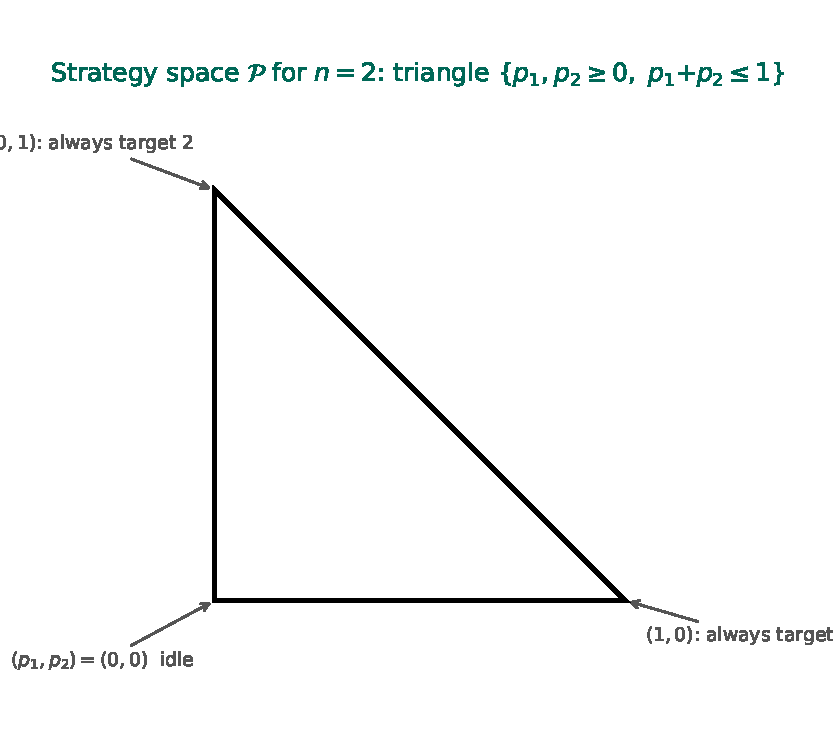
\includegraphics[width=\linewidth]{figures/simplex_2t.pdf}
\end{column}
\begin{column}{0.45\textwidth}
\begin{itemize}\small
  \item With $n=2$ targets and one resource (which may be idle), the coverage space is the triangle
  \[
  \cP=\{(p_1,p_2):p_1\geq 0,\;p_2\geq 0,\;p_1+p_2\leq 1\}.
  \]
  \item Vertex $(1,0)$: always cover target 1.
  \item Vertex $(0,1)$: always cover target 2.
  \item Vertex $(0,0)$: resource is idle (no target defended).
  \item $\cP$ is a convex polytope -- the same 2D triangle used in Balcan et al., Figure 1.
\end{itemize}
\end{column}
\end{columns}
\end{frame}


\begin{frame}{Attacker types and best response}
\begin{itemize}
  \item An attacker \impcompterm{type} $\alpha$ is specified by utilities $u_\alpha^c(i), u_\alpha^u(i)\in[-1,1]$:
        \[U_\alpha(i,\pvec)\;=\;u_\alpha^c(i)\,p_i\;+\;u_\alpha^u(i)\,(1-p_i).\]
  \item Observing $\pvec$, type $\alpha$ \impterm{best-responds}:
        \[ b_\alpha(\pvec)\;=\;\argmax_{i\in N}\,U_\alpha(i,\pvec).\]
  \item Per-round payoff to the defender when type $\alpha$ attacks:
        \[ U_d\bigl(b_\alpha(\pvec),\pvec\bigr).\]
\end{itemize}
\vspace{6pt}
\begin{alertblock}{The technical difficulty}
The best-response operator $b_\alpha(\cdot)$ is piecewise constant in $\pvec$.
Hence the defender's loss is \textbf{not} linear or continuous in $\pvec$.
\end{alertblock}
\end{frame}


\begin{frame}{Repeated game and regret}
\begin{itemize}
  \item Time horizon $T$ is known. An \impterm{oblivious} adversary fixes a sequence $\avec=a_1,\dots,a_T\in K^T$ before the game starts.
  \item At each round $t$:
    \begin{enumerate}\small
      \item Defender commits $\pvec_t\in\cP$.
      \item Attacker $a_t$ plays $b_{a_t}(\pvec_t)$; defender receives $U_d(b_{a_t}(\pvec_t),\pvec_t)$.
      \item \impcompterm{Full information feedback}: defender observes $a_t$ (and, first time $\alpha$ is seen, its full utility).
    \end{enumerate}
  \item Benchmark -- \impterm{best fixed coverage in hindsight}:
        \[ \pvec^{*}\;=\;\argmax_{\pvec\in\cP}\;\sum_{t=1}^T U_d\bigl(b_{a_t}(\pvec),\pvec\bigr).\]
\end{itemize}
\pause
\vspace{-4pt}
\begin{greenblock}{Expected regret}
\[
\mathrm{Regret}(T)\;=\;\sum_{t=1}^{T}U_d\bigl(b_{a_t}(\pvec^{*}),\pvec^{*}\bigr)\;-\;\EE\!\Bigl[\sum_{t=1}^{T}U_d\bigl(b_{a_t}(\pvec_t),\pvec_t\bigr)\Bigr].
\]
\end{greenblock}
\end{frame}


\begin{frame}{Balcan, Blum, Haghtalab, Procaccia (2015) -- known $K$}
\begin{greenblock}{Theorem 5.1 (Balcan et al.)}
If $K$ with $|K|=k$ is \emph{known} upfront and feedback is full information, there is an online algorithm achieving
\[
\EE[\mathrm{Regret}(T)]\;\le\;O\!\left(\sqrt{T\cdot n^2\cdot k\cdot\log(nk)}\right).
\]
\end{greenblock}
\pause
\begin{itemize}
  \item Proof technique: partition $\cP$ into finitely many best-response regions, enumerate the \impcompterm{$\epsilon$-approximate extreme point set} $\cE(K;\epsilon)$, run an online learning subroutine over $\cE$.
  \item Lower bound (Thm.\ 7.1): unrestricted $|K|$ $\Rightarrow$ $\Omega(T)$ regret.
\end{itemize}
\pause
\vspace{3pt}
\begin{alertblock}{Our extension}
$|K|$ unknown a priori, but we are given a constant $\Kmax$ with $|K|\le\Kmax$.
New types reveal their full utility when first observed.
\end{alertblock}
\end{frame}


% ============================================================================
\section{Proof, algorithm, and results}
% ============================================================================

\begin{frame}{Primer: half-spaces and convex polytopes}
\begin{itemize}
\item A \impterm{half-space} in $\mathbb{R}^n$ is $\{\pvec:\bm a^{\top}\pvec\le b\}$.
\item A \impcompterm{convex polytope} is a bounded intersection of finitely many half-spaces.
\item For each attacker type $\alpha$ and target $i$,
      \[
      \cP_i^\alpha\;=\;\{\pvec\in\cP\,:\,b_\alpha(\pvec)=i\}
      \]
      is itself a convex polytope (defined by the pairwise linear inequalities $U_\alpha(i,\pvec)\ge U_\alpha(j,\pvec)$).
\item For a response profile $\sigma:C\to N$,
      \[\cP_\sigma(C)\;=\;\bigcap_{\alpha\in C}\cP_{\sigma(\alpha)}^\alpha\]
      is again a convex polytope.
\end{itemize}
\end{frame}


\begin{frame}{A concrete example for $n=2$: one best-response cut}
\begin{columns}[T]
\begin{column}{0.55\textwidth}
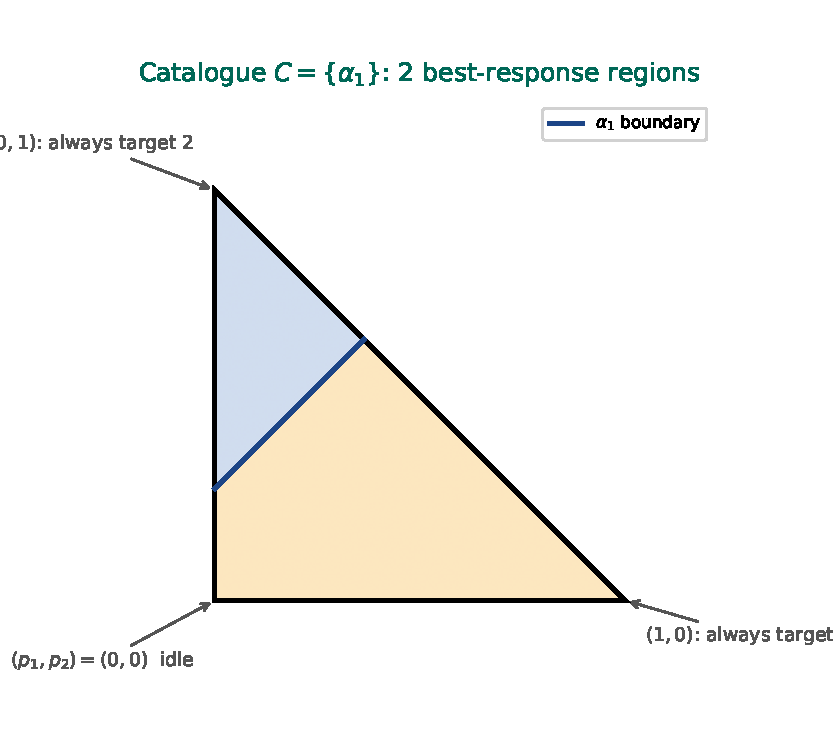
\includegraphics[width=\linewidth]{figures/partition_2t_1.pdf}
\end{column}
\begin{column}{0.45\textwidth}
\begin{itemize}\small
\item With $n=2$ and an idle option, $\cP$ is the triangle $\{p_1,p_2\geq 0,\;p_1{+}p_2\leq 1\}$.
\item For one attacker $\alpha_1$, $U_{\alpha_1}(1,\pvec)=U_{\alpha_1}(2,\pvec)$ is a single line in $(p_1,p_2)$-space -- one \impterm{best-response boundary}.
\item On one side of the line $\alpha_1$ attacks target $1$; on the other, target $2$.
\item $\cP$ is split into \textbf{2 convex polytopes}.
\end{itemize}
\end{column}
\end{columns}
\end{frame}


\begin{frame}{Adding more types refines the partition}
\begin{columns}[T]
\begin{column}{0.52\textwidth}
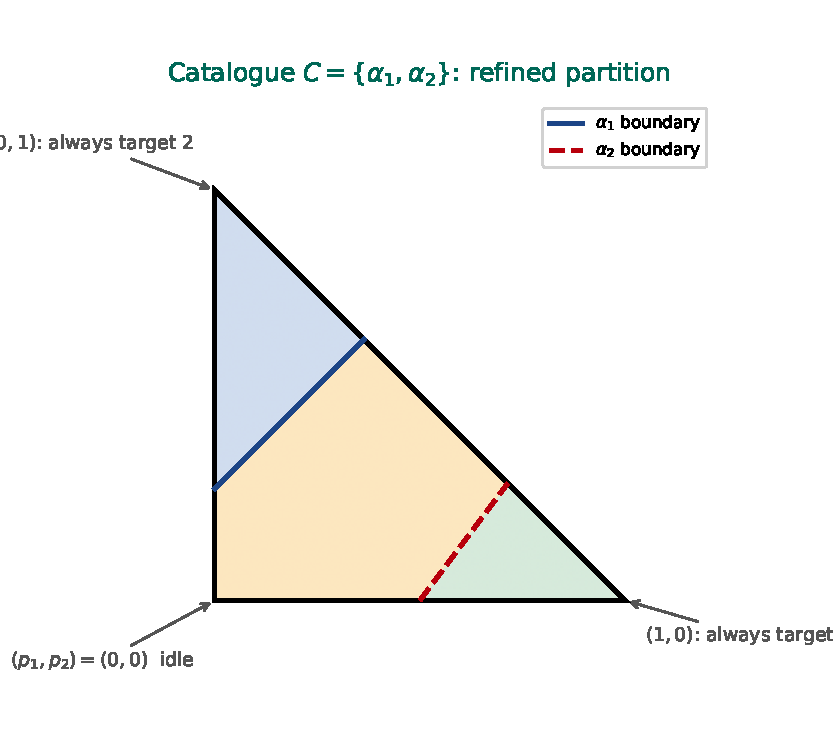
\includegraphics[width=\linewidth]{figures/partition_2t_2.pdf}\\[-2pt]
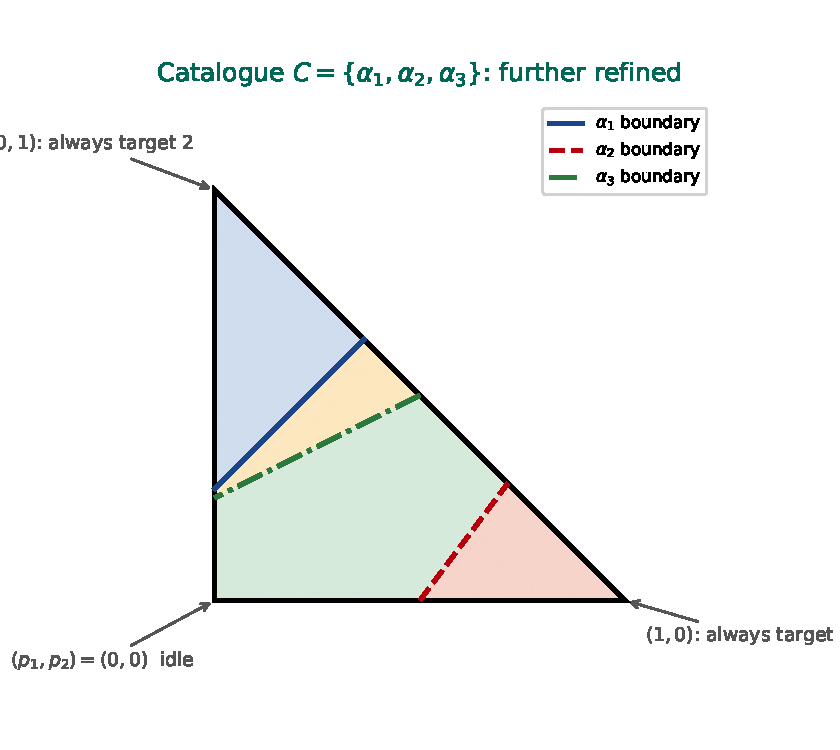
\includegraphics[width=\linewidth]{figures/partition_2t_3.pdf}
\end{column}
\begin{column}{0.48\textwidth}
\begin{itemize}\small
\item Each new type $\alpha$ adds $\binom{n}{2}$ linear boundaries ($=1$ line when $n=2$).
\item Existing polytopes get \impcompterm{sliced}, never lost; the refined partition is still a collection of convex polytopes.
\item Within any $\cP_\sigma(C)$, the best response of every $\alpha\in C$ is fixed $\Rightarrow$ the defender's payoff is \impterm{linear} in $\pvec$ on that region.
\end{itemize}
\end{column}
\end{columns}
\end{frame}


\begin{frame}{The $\cE(C)$ set of extreme points}
\begin{columns}[T]
\begin{column}{0.42\textwidth}
\vspace{4pt}
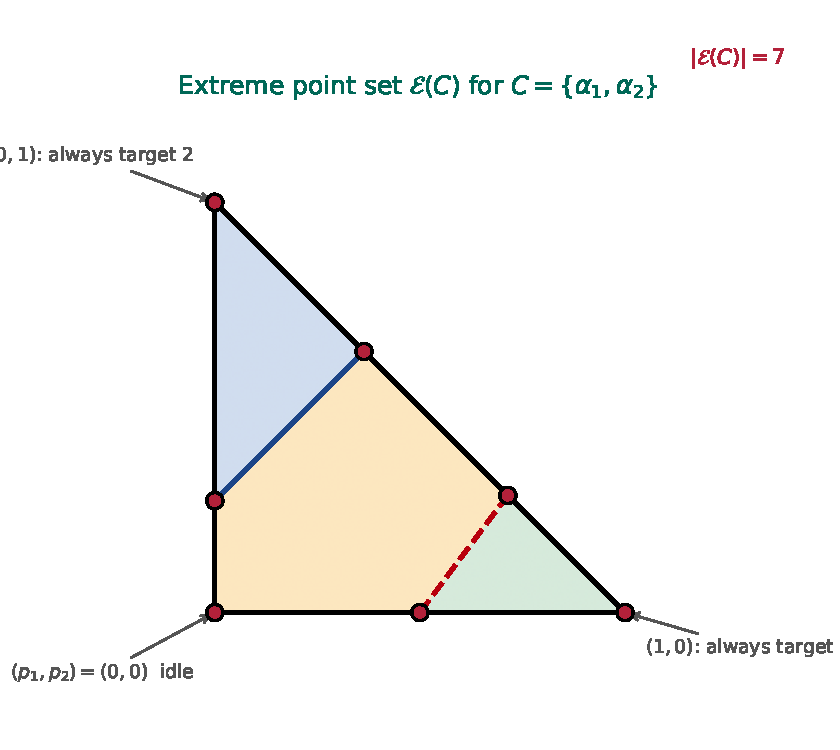
\includegraphics[width=\linewidth]{figures/extreme_points_2t.pdf}
\end{column}
\begin{column}{0.58\textwidth}
\scriptsize
\begin{itemize}
\item Within each $\cP_\sigma(C)$, the defender's payoff is linear in $\pvec$ $\Rightarrow$ its maximum is attained at a \impcompterm{vertex} of $\cP_\sigma(C)$.
\item Define $\cE(C;\epsilon)$ = the $\epsilon$-approximate vertices of all $\cP_\sigma(C)$.
\item Key facts (Balcan et al., Lemmas 4.3, 4.4):
\[
\max_{\pvec\in\cE(C)}\!\sum_t\! U_d(b_{a_t}(\pvec),\pvec)\ge\max_{\pvec\in\cP}\!\sum_t\! U_d(b_{a_t}(\pvec),\pvec)-2\epsilon T
\]
\[
|\cE(C;\epsilon)|\le O\!\bigl((2^n+|C|n^2)^n\cdot n^{|C|}\bigr)
\]
\end{itemize}
\end{column}
\end{columns}
\end{frame}


\begin{frame}{$\cE(C)$ grows as new types are discovered}
\begin{center}
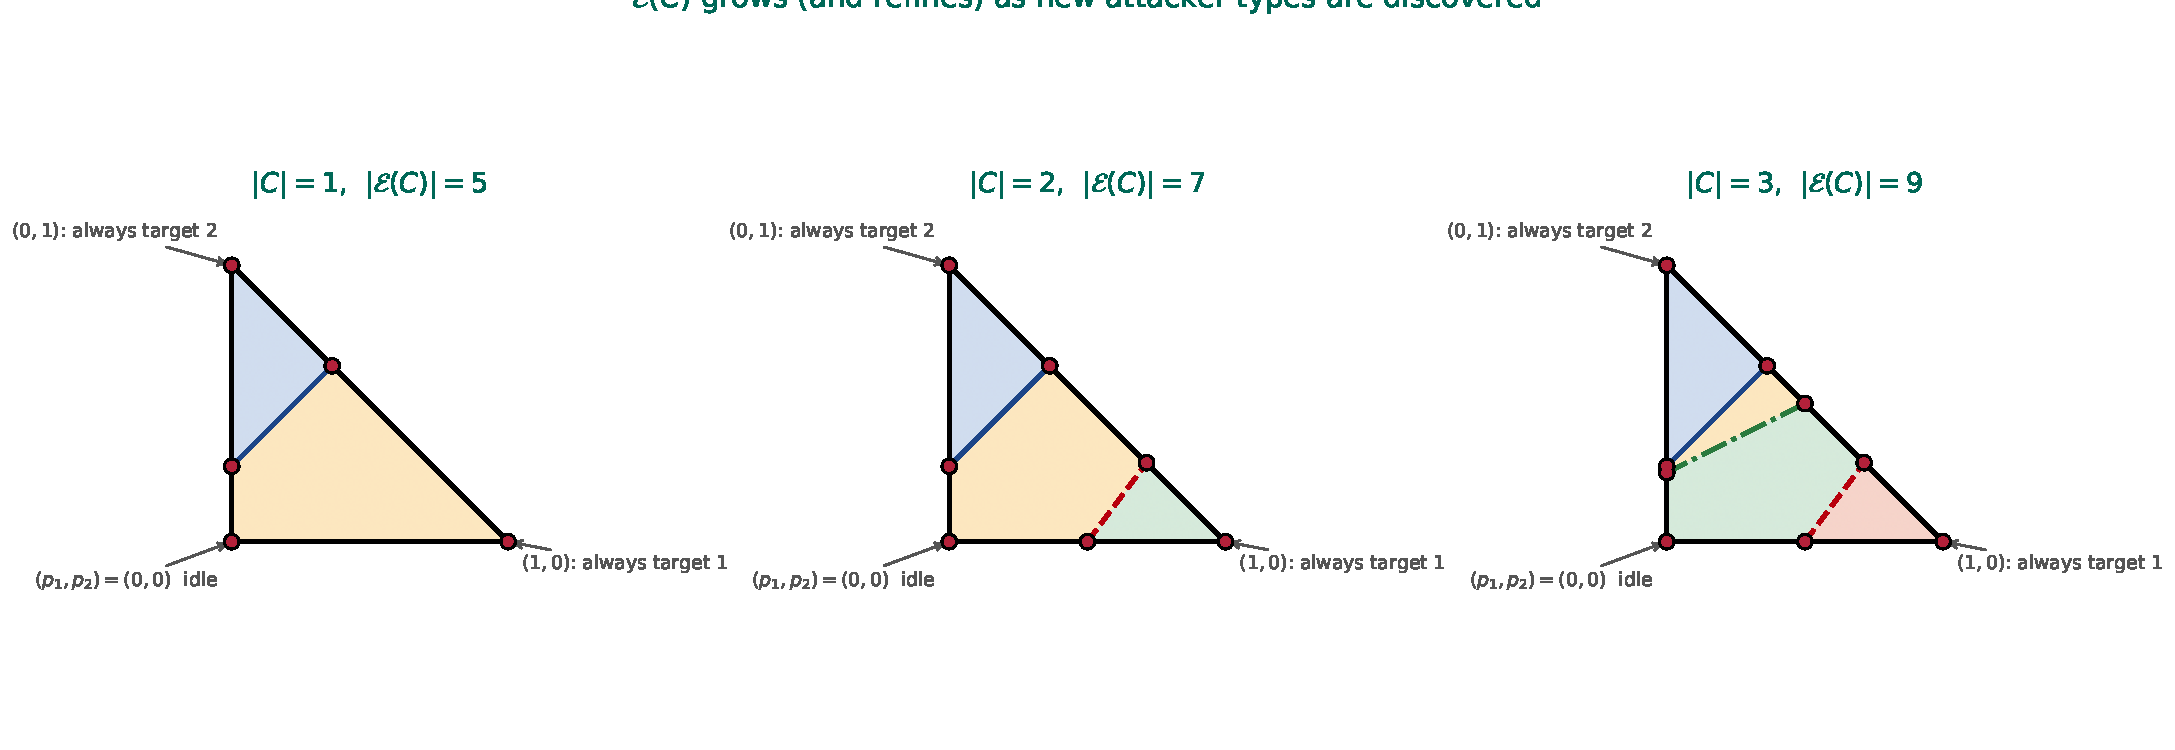
\includegraphics[width=0.94\linewidth]{figures/eset_growth_2t.pdf}
\end{center}
\vspace{-4pt}
\begin{itemize}\small
\item Each new type adds a best-response line and hence new vertices.
\item $|\cE(C_i)|$ is bounded uniformly by $N_{\max}:=|\cE(C;\epsilon)|$ at $|C|=\Kmax$.
\item The analysis works on the \emph{current} $\cE(C)$ at each round -- no need to anticipate future types.
\end{itemize}
\end{frame}


\begin{frame}{Our main theorem}
\begin{greenblock}{Theorem (unknown $K$, full information)}
Let $K$ be an unknown set of attacker types with $|K|\le\Kmax$.
For full-information feedback and any oblivious adversarial sequence $\avec\in K^T$,
there is an online algorithm whose expected regret satisfies
\[
\EE[\mathrm{Regret}(T)]\;\le\;O\!\left(\sqrt{T\cdot\Kmax\cdot(n^2+\Kmax\log n)}\right).
\]
\end{greenblock}
\vspace{4pt}
\begin{itemize}
\item Same form as Balcan et al.\ Theorem 5.1, with $k$ replaced by $\Kmax$.
\item For $\Kmax=O(1)$ the rate matches the known-$K$ rate up to log factors.
\item Instance-adaptive: if only $K'<\Kmax$ types actually appear, the bound tightens to $O(\sqrt{TK'(n^2+\Kmax\log n)})$.
\end{itemize}
\end{frame}


\begin{frame}{Proof idea in one picture}
\begin{center}
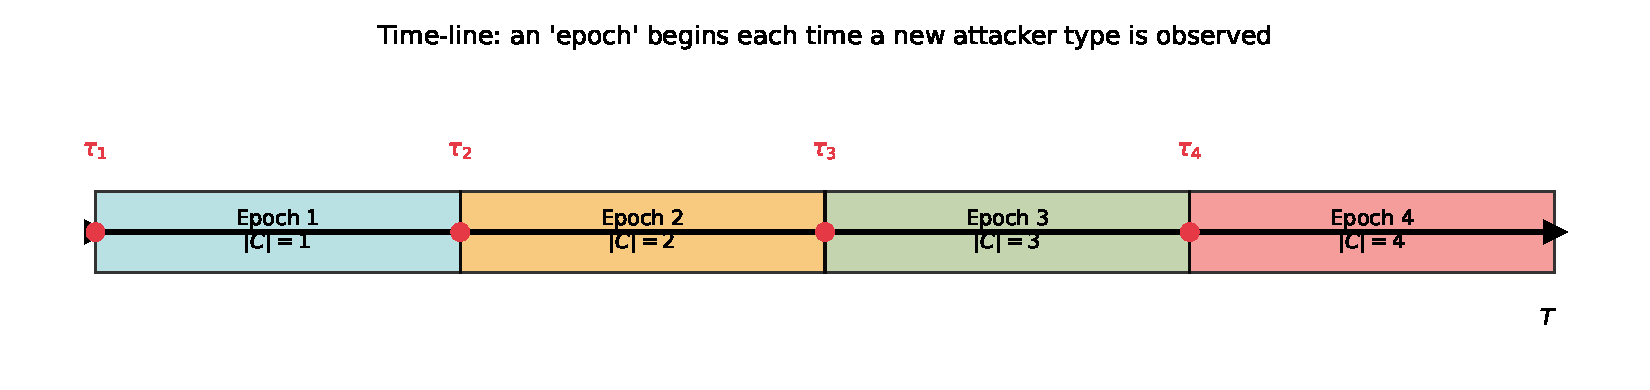
\includegraphics[width=\linewidth]{figures/epoch_decomposition.pdf}
\end{center}
\vspace{-10pt}
\begin{enumerate}\small
\item Split $[1,T]$ into \impcompterm{epochs}: epoch $i$ starts right after the $i$-th new type is discovered and ends before the $(i{+}1)$-st.
\item Within an epoch, the catalogue $C_i$ is fixed; run an online learning subroutine on $\cE(C_i)$.
\item Apply Balcan et al.'s within-epoch analysis (regret bound + Lemma 4.3) to each epoch.
\item Sum over at most $\Kmax$ epochs using \impterm{Cauchy--Schwarz}.
\item Absorb $K'\le\Kmax$ \emph{discovery rounds} into a $2\Kmax$ additive term.
\end{enumerate}
\end{frame}


\begin{frame}{Proof -- within-epoch regret}
\begin{block}{Online learning black-box (Balcan et al.\ Proposition 1)}
For any fixed expert set $\cE_i$ and any $L_i$ rounds, there is an online learning algorithm whose expected regret satisfies
\[
\max_{\pvec\in\cE_i}\sum_{t\in\text{Ep.}_i}\!U_d(b_{a_t}(\pvec),\pvec)\;-\;\EE\!\left[\sum_{t\in\text{Ep.}_i}\!U_d(b_{a_t}(\pvec_t),\pvec_t)\right]\;\le\;c_1\sqrt{L_i\log|\cE_i|}.
\]
\end{block}
\pause
\begin{block}{Approximation by extreme points (Lemma 4.3)}
Inside epoch $i$ the sequence only uses types in $C_i$, so
\[
\max_{\pvec\in\cE_i}\!\sum_{t\in\text{Ep.}_i}U_d(b_{a_t}(\pvec),\pvec)\;\ge\;\sum_{t\in\text{Ep.}_i}U_d(b_{a_t}(\pvec^{*}),\pvec^{*})-2\epsilon L_i.
\]
\end{block}
\end{frame}


\begin{frame}{Proof -- combining the two within an epoch}
Chaining the two inequalities from the previous slide gives, for every epoch $i$:
\[
\EE\!\left[\sum_{t\in\text{Ep.}_i}\!U_d(b_{a_t}(\pvec_t),\pvec_t)\right]\;\ge\;\sum_{t\in\text{Ep.}_i}U_d(b_{a_t}(\pvec^{*}),\pvec^{*})\;-\;2\epsilon L_i\;-\;c_1\sqrt{L_i\log|\cE_i|}.
\]
\vspace{4pt}
\begin{itemize}\small
\item The left-hand side is the algorithm's expected utility on epoch $i$.
\item The right-hand side compares against the global benchmark $\pvec^{*}$ restricted to epoch $i$.
\item The $2\epsilon L_i$ term is the Lemma-4.3 approximation loss.
\item The $c_1\sqrt{L_i\log|\cE_i|}$ term is the within-epoch regret of the online learning subroutine.
\end{itemize}
\end{frame}


\begin{frame}{Proof -- summing epochs with Cauchy--Schwarz}
Summing the per-epoch inequality over $i=1,\dots,K'$, using $\sum_i L_i\le T$ and a discovery-round term $2\Kmax$:
\[
\EE[\mathrm{Regret}(T)]\;\le\;2\Kmax\;+\;2\epsilon T\;+\;c_1\sqrt{\log N_{\max}}\sum_{i=1}^{K'}\sqrt{L_i}.
\]
\pause
By Cauchy--Schwarz,
\[
\sum_{i=1}^{K'}\sqrt{L_i}\;\le\;\sqrt{K'\cdot\textstyle\sum_i L_i}\;\le\;\sqrt{\Kmax\,T}.
\]
\pause
Plug $\epsilon=1/\sqrt T$ and $\log N_{\max}=O(n^2+\Kmax\log n)$ to obtain
\[
\EE[\mathrm{Regret}(T)]\;\le\;O\!\left(\sqrt{T\cdot\Kmax\cdot(n^2+\Kmax\log n)}\right).\qquad\square
\]
\end{frame}


\begin{frame}{Regime in which the bound is meaningful}
\begin{itemize}
\item The bound is sublinear in $T$ iff $\Kmax\cdot(n^2+\Kmax\log n)=o(T)$.
\item Equivalently,
      \[
      \Kmax\;=\;o\!\left(\min\!\left\{\tfrac{T}{n^2},\,\sqrt{\tfrac{T}{\log n}}\right\}\right).
      \]
\item $\Kmax=O(1)$: $\tilde O(n\sqrt T)$ for any $n\le T^{1/2}$.
\item $\Kmax=\Theta(n^c)$: sublinear as long as $T=\omega(n^{c+2})$.
\item For $\Kmax\gtrsim T/n^2$ the upper bound becomes trivial -- matches Balcan et al.'s linear-regret lower bound on the unbounded side.
\end{itemize}
\end{frame}


\begin{frame}{The \textsc{Grow-Catalogue} algorithm}
\small
\begin{block}{Algorithm (full information)}
\begin{enumerate}
\item $C\gets\emptyset$, $\cE\gets\emptyset$, $\epsilon\gets 1/\sqrt T$.
\item For $t=1,\dots,T$:
\begin{itemize}\small
\item If $\cE=\emptyset$, play uniform $\pvec_{\text{def}}$; else sample $\pvec_t\sim\qvec_t$ where $\qvec_t$ is the current Hedge distribution over $\cE$.
\item Observe $a_t$.
\item \textbf{New type} ($a_t\notin C$): add $a_t$ (and its utility) to $C$, \impcompterm{recompute} $\cE\gets\cE(C;\epsilon)$, restart Hedge on the new $\cE$.
\item Else: compute $\ell_t(\pvec)=-U_d(b_{a_t}(\pvec),\pvec)$ for all $\pvec\in\cE$, update Hedge with anytime learning rate $\eta_{t_{\text{loc}}}=\sqrt{\log|\cE|/t_{\text{loc}}}$.
\end{itemize}
\end{enumerate}
\end{block}
\begin{itemize}\small
\item We implement two variants: \textbf{total recomputation} and \textbf{incremental} (reuse surviving extreme points' weights). Same regret, different wall-clock.
\item The anytime learning rate gives a $\sqrt{L_i}$-per-epoch guarantee without knowing $L_i$ in advance.
\end{itemize}
\end{frame}


\begin{frame}{Experiment design}
\begin{greenblock}{Staggered-uniform adversary}
Partition $[0,T)$ into $\Kmax$ phases of length $T/\Kmax$. In phase $i$ the attacker is drawn uniformly at random from $\{\alpha_1,\dots,\alpha_i\}$:
\begin{itemize}\small
\item phase $1$: only $\alpha_1$;
\item phase $2$: $\{\alpha_1,\alpha_2\}$ each w.p.\ $\tfrac12$;
\item phase $i$: each of the $i$ revealed types with prob.\ $\tfrac1i$.
\end{itemize}
\end{greenblock}
\begin{itemize}\small
\item $n=3$, $\Kmax=4$, $T=4000$, averaged over 40 random instances.
\item Old types keep arriving after each reveal $\Rightarrow$ the benchmark $\pvec^{*}$ is a genuine compromise, not a specialist.
\item Reveals happen at rounds $0,\,1000,\,2000,\,3000$.
\end{itemize}
\end{frame}


\begin{frame}{Result 1: per-round regret vs iteration}
\begin{center}
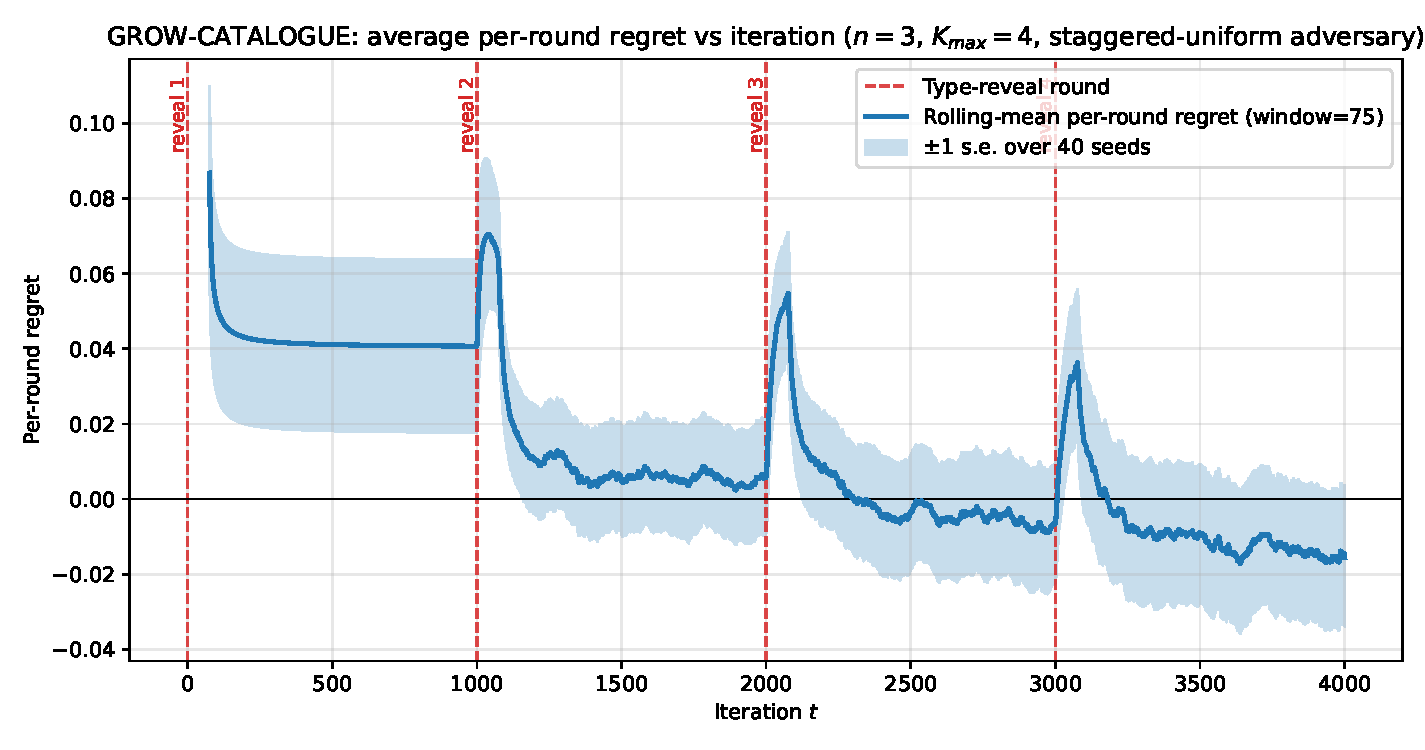
\includegraphics[width=0.78\linewidth]{figures/avg_regret_per_iter.pdf}
\end{center}
\vspace{-10pt}
\begin{itemize}\small
\item Clear \impterm{spikes} at each reveal round where a new type first appears, followed by re-convergence.
\item Spikes shrink over time: more types already known $\Rightarrow$ each reveal is less disruptive.
\end{itemize}
\end{frame}


\begin{frame}{Result 2: global average regret $\mathrm{Regret}(t)/t$}
\begin{center}
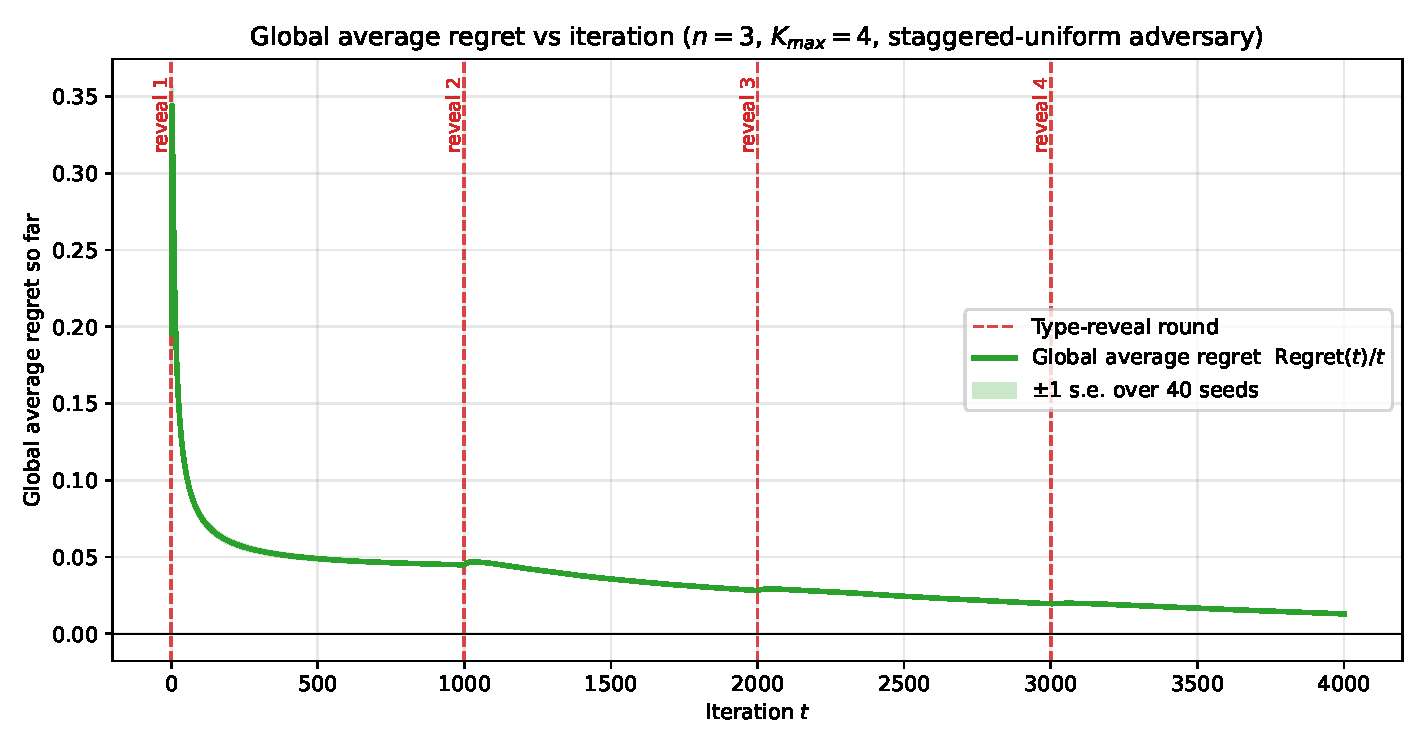
\includegraphics[width=0.84\linewidth]{figures/global_avg_regret.pdf}
\end{center}
\vspace{-8pt}
\begin{itemize}\small
\item Global average regret tends to $0$ from above, consistent with the sublinear regret theorem.
\item Tiny bumps at reveal rounds confirm the epoch structure.
\end{itemize}
\end{frame}


% ---------------- Closing ----------------

\begin{frame}{Take-aways}
\begin{itemize}\small
\item Sequential (Stackelberg) SSGs are the \impterm{harder} model -- the right target for a worst-case bound.
\item Unknown $K$ with a known bound $\Kmax$: we prove
\[
\EE[\mathrm{Regret}(T)]\;=\;O\!\left(\sqrt{T\cdot\Kmax\cdot(n^2+\Kmax\log n)}\right),
\]
the same form as Balcan et al.\ with $k\to\Kmax$.
\item The bound is meaningful as long as $\Kmax\cdot(n^2+\Kmax\log n)\ll T$.
\item Experiments on a staggered-uniform adversary confirm sublinear regret with visible spikes at discovery rounds.
\end{itemize}
\pause
\begin{block}{Future directions}
\begin{itemize}\small
\item \textbf{Partial-information} feedback (bandit version), needing adaptive barycentric spanners.
\item \textbf{Adaptive adversary} under partial info (Balcan et al.'s explicit open problem).
\item Tightening the logarithmic dependence on $\Kmax$ via sleeping-experts techniques.
\end{itemize}
\end{block}
\end{frame}


\begin{frame}[allowframebreaks]{References}
\footnotesize
\begin{thebibliography}{9}
\bibitem{bbhp2015} M.-F.\ Balcan, A.\ Blum, N.\ Haghtalab, A.\ D.\ Procaccia. Commitment without regrets: online learning in Stackelberg security games. EC 2015.
\bibitem{cesabianchi} N.\ Cesa-Bianchi, G.\ Lugosi. Prediction, Learning, and Games. Cambridge University Press, 2006.
\bibitem{bhp2014} A.\ Blum, N.\ Haghtalab, A.\ D.\ Procaccia. Learning optimal commitment to overcome insecurity. NeurIPS 2014.
\bibitem{tambe} M.\ Tambe. Security and Game Theory: Algorithms, Deployed Systems, Lessons Learned. CUP 2012.
\bibitem{kiekintveld} C.\ Kiekintveld, J.\ Marecki, M.\ Tambe. Approximation methods for infinite Bayesian Stackelberg games. AAMAS 2011.
\bibitem{pita} J.\ Pita et al. Robust solutions to Stackelberg games with bounded rationality and limited observations. AIJ 2010.
\bibitem{yang} R.\ Yang et al. Adaptive resource allocation for wildlife protection. AAMAS 2014.
\end{thebibliography}
\end{frame}


\begin{frame}
  \vfill
  \centering
  {\Huge\color{darkgreen}\textbf{Thank you}}\par
  \vspace{0.5em}
  {\large\color{blueprimary}Questions?}
  \vfill
\end{frame}

\end{document}
